%----------------------------------------------------------------------------------------
%	PACKAGES AND OTHER DOCUMENT CONFIGURATIONS
%----------------------------------------------------------------------------------------

\documentclass[12pt]{article}
\renewcommand{\baselinestretch}{1.0} 
\usepackage[T1]{fontenc}
\usepackage{graphicx}
\usepackage{amssymb}
%%%%%%%%%%%%%%%%%%%%%%%%%%%%%%%%%%%%%%%%%
% Lachaise Assignment
% Structure Specification File
% Version 1.0 (26/6/2018)
%
% This template originates from:
% http://www.LaTeXTemplates.com
%
% Authors:
% Marion Lachaise & François Févotte
% Vel (vel@LaTeXTemplates.com)
%
% License:
% CC BY-NC-SA 3.0 (http://creativecommons.org/licenses/by-nc-sa/3.0/)
% 
%%%%%%%%%%%%%%%%%%%%%%%%%%%%%%%%%%%%%%%%%

%----------------------------------------------------------------------------------------
%	PACKAGES AND OTHER DOCUMENT CONFIGURATIONS
%----------------------------------------------------------------------------------------

\usepackage{amsmath,amsfonts,stmaryrd,amssymb} % Math packages

\usepackage{enumerate} % Custom item numbers for enumerations

\usepackage[ruled]{algorithm2e} % Algorithms

\usepackage[framemethod=tikz]{mdframed} % Allows defining custom boxed/framed environments

\usepackage{listings} % File listings, with syntax highlighting
\lstset{
	basicstyle=\ttfamily, % Typeset listings in monospace font
}

%----------------------------------------------------------------------------------------
%	DOCUMENT MARGINS
%----------------------------------------------------------------------------------------

\usepackage{geometry} % Required for adjusting page dimensions and margins

\geometry{
	paper=a4paper, % Paper size, change to letterpaper for US letter size
	top=2.5cm, % Top margin
	bottom=3cm, % Bottom margin
	left=2.5cm, % Left margin
	right=2.5cm, % Right margin
	headheight=14pt, % Header height
	footskip=1.5cm, % Space from the bottom margin to the baseline of the footer
	headsep=1.2cm, % Space from the top margin to the baseline of the header
	%showframe, % Uncomment to show how the type block is set on the page
}

%----------------------------------------------------------------------------------------
%	FONTS
%----------------------------------------------------------------------------------------

\usepackage[utf8]{inputenc} % Required for inputting international characters
\usepackage[T1]{fontenc} % Output font encoding for international characters

\usepackage{XCharter} % Use the XCharter fonts

%----------------------------------------------------------------------------------------
%	COMMAND LINE ENVIRONMENT
%----------------------------------------------------------------------------------------

% Usage:
% \begin{commandline}
%	\begin{verbatim}
%		$ ls
%		
%		Applications	Desktop	...
%	\end{verbatim}
% \end{commandline}

\mdfdefinestyle{commandline}{
	leftmargin=10pt,
	rightmargin=10pt,
	innerleftmargin=15pt,
	middlelinecolor=black!50!white,
	middlelinewidth=2pt,
	frametitlerule=false,
	backgroundcolor=black!5!white,
	frametitle={Command Line},
	frametitlefont={\normalfont\sffamily\color{white}\hspace{-1em}},
	frametitlebackgroundcolor=black!50!white,
	nobreak,
}

% Define a custom environment for command-line snapshots
\newenvironment{commandline}{
	\medskip
	\begin{mdframed}[style=commandline]
}{
	\end{mdframed}
	\medskip
}

%----------------------------------------------------------------------------------------
%	FILE CONTENTS ENVIRONMENT
%----------------------------------------------------------------------------------------

% Usage:
% \begin{file}[optional filename, defaults to "File"]
%	File contents, for example, with a listings environment
% \end{file}

\mdfdefinestyle{file}{
	innertopmargin=1.6\baselineskip,
	innerbottommargin=0.8\baselineskip,
	topline=false, bottomline=false,
	leftline=false, rightline=false,
	leftmargin=2cm,
	rightmargin=2cm,
	singleextra={%
		\draw[fill=black!10!white](P)++(0,-1.2em)rectangle(P-|O);
		\node[anchor=north west]
		at(P-|O){\ttfamily\mdfilename};
		%
		\def\l{3em}
		\draw(O-|P)++(-\l,0)--++(\l,\l)--(P)--(P-|O)--(O)--cycle;
		\draw(O-|P)++(-\l,0)--++(0,\l)--++(\l,0);
	},
	nobreak,
}

% Define a custom environment for file contents
\newenvironment{file}[1][File]{ % Set the default filename to "File"
	\medskip
	\newcommand{\mdfilename}{#1}
	\begin{mdframed}[style=file]
}{
	\end{mdframed}
	\medskip
}

%----------------------------------------------------------------------------------------
%	NUMBERED QUESTIONS ENVIRONMENT
%----------------------------------------------------------------------------------------

% Usage:
% \begin{question}[optional title]
%	Question contents
% \end{question}

\mdfdefinestyle{question}{
	innertopmargin=1.2\baselineskip,
	innerbottommargin=0.8\baselineskip,
	roundcorner=5pt,
	nobreak,
	singleextra={%
		\draw(P-|O)node[xshift=1em,anchor=west,fill=white,draw,rounded corners=5pt]{%
		Question \theQuestion\questionTitle};
	},
}

\newcounter{Question} % Stores the current question number that gets iterated with each new question

% Define a custom environment for numbered questions
\newenvironment{question}[1][\unskip]{
	\bigskip
	\stepcounter{Question}
	\newcommand{\questionTitle}{~#1}
	\begin{mdframed}[style=question]
}{
	\end{mdframed}
	\medskip
}

%----------------------------------------------------------------------------------------
%	WARNING TEXT ENVIRONMENT
%----------------------------------------------------------------------------------------

% Usage:
% \begin{warn}[optional title, defaults to "Warning:"]
%	Contents
% \end{warn}

\mdfdefinestyle{warning}{
	topline=false, bottomline=false,
	leftline=false, rightline=false,
	nobreak,
	singleextra={%
		\draw(P-|O)++(-0.5em,0)node(tmp1){};
		\draw(P-|O)++(0.5em,0)node(tmp2){};
		\fill[black,rotate around={45:(P-|O)}](tmp1)rectangle(tmp2);
		\node at(P-|O){\color{white}\scriptsize\bf !};
		\draw[very thick](P-|O)++(0,-1em)--(O);%--(O-|P);
	}
}

% Define a custom environment for warning text
\newenvironment{warn}[1][Warning:]{ % Set the default warning to "Warning:"
	\medskip
	\begin{mdframed}[style=warning]
		\noindent{\textbf{#1}}
}{
	\end{mdframed}
}

%----------------------------------------------------------------------------------------
%	INFORMATION ENVIRONMENT
%----------------------------------------------------------------------------------------

% Usage:
% \begin{info}[optional title, defaults to "Info:"]
% 	contents
% 	\end{info}

\mdfdefinestyle{info}{%
	topline=false, bottomline=false,
	leftline=false, rightline=false,
	nobreak,
	singleextra={%
		\fill[black](P-|O)circle[radius=0.4em];
		\node at(P-|O){\color{white}\scriptsize\bf i};
		\draw[very thick](P-|O)++(0,-0.8em)--(O);%--(O-|P);
	}
}

% Define a custom environment for information
\newenvironment{info}[1][Info:]{ % Set the default title to "Info:"
	\medskip
	\begin{mdframed}[style=info]
		\noindent{\textbf{#1}}
}{
	\end{mdframed}
}
 % Include the file specifying the document structure and custom commands

%----------------------------------------------------------------------------------------
%	ASSIGNMENT INFORMATION
%----------------------------------------------------------------------------------------

\title{Image classification using Convolutional Neural Networks \\ Gradient descent optimization
algorithms} % Title of the assignment

\author{Ciprian-Mihai Ceausescu\\ \texttt{ciprian-mihai.ceausescu@my.fmi.unibuc.ro}} % Author name and email address

\date{University of Bucharest --- \today} % University, school and/or department name(s) and a date

%----------------------------------------------------------------------------------------

\begin{document}

\maketitle % Print the title

%----------------------------------------------------------------------------------------
%	Introduction
%----------------------------------------------------------------------------------------

\section*{Introduction}

\hspace{10mm}In Deep Learning, a Convolutional Neural Network, CNN is a class of deep, feed-forward Artificial Neural Networks, most commonly applied to analyzing visual imagery. An Artificial Neural Network, ANN, the base definition of a Convolutional Neural Network, also known as a connectionist system is defined as a biological neural network that constitute the brain of an animal. ANN is also called a feed-forward network and it has the goal to make an approximation of some function \textit{f}. \\
\hspace*{10mm}As example, we can take a classifier, $y=f(x)$ that will map an input \textit{x} to a category \textit{y}. A feed-forward neural network defines a mapping function $y=f(x;\theta)$ and learns the value of the parameters $\theta$ that will result in the best function approximation.\\
\hspace*{10mm}Convolutional Neural Networks models are called feed-forward because the information flows\\ throught the function being evaluated from \textit{x}, throught the intermediate computations used to define the function \textit{f} and finally to the output \textit{y}. A very important aspect is that there we have not any feedback connections in the networks outputs of the model that are fed back into itself. These feed-forward neural networks are called networks because they are typically represented by computing together many different functions. The model is associated with a directed acyclic graph describing how the functions are composed together in order to get the result of training. As an example, we can take three functions, 
$f^{(1)}, f^{(2)}, f^{(3)}$ that are connected in a chain, to form $f(x)=f^{(3)}(f^{(2)}(f^{(1)}(x)))$. The overall length of the chain dives the \textit{depth} of the model, and so, a Convolutional Neural Network is a Deep Learning model.

%----------------------------------------------------------------------------------------
%	Training of Convolutional Neural Network
%----------------------------------------------------------------------------------------

\section*{Training of Convolutional Neural Networks} 
\hspace*{10mm}The training of Convolutional Neural Networks consists of defining three main components:
\begin{enumerate}[1.]
	\item \textbf{Convolutional layers} - which apply various convolution channels to the information. For every subregion, the layer plays out a lot of mathematical operations to create a solitary incentive in the yield include delineate. Convolutional layers at that point ordinarily apply a ReLU activation function to the yield to bring nonlinearities into the model.
	\item \textbf{Pooling layers} - which downsample the picture information removed by the convolutional layers to diminish the dimensionality of the component delineate request to diminish preparing time. A normally utilized pooling calculation is max pooling, which extricates subregions of the element outline, (2x2-pixel tiles), keeps their most extreme esteem, and disposes of every other values.
	\item \textbf{Dense or fully connected layers} - which perform arrangement on the highlights extricated by the convolutional layers and downsampled by the pooling layers. In a thick layer, each hub in the layer is associated with each hub in the previous layer.
\end{enumerate}
\hspace*{10mm} \\ \hspace*{10mm}Mainly, a Convolutional Neural Network is created using a pile of convolutional modules that perform include extraction. Every module comprises of a convolutional layer pursued by a pooling layer. The last convolutional module is trailed by at least one thick layers that perform characterization. The last thick layer in a Convolutional Neural Network contains a solitary hub for each objective class in the model (all the conceivable classes the model may anticipate), with a softmax activation function to create a value between 0– 1 for every hub (the total of all these softmax values is equivalent to 1). We can translate the softmax values for a given picture as relative estimations of how likely it is that the picture falls into each objective class.
\\ \hspace*{10mm} \\ \hspace*{10mm}For training a Convolutional Neural Network are defined some important elements regarding the amount of data used and steps that are done:
\begin{enumerate}[1.]
	\item \textbf{Epoch} - is a single step in training a Neural Network. In other words when a Neural Network is trained on every training samples only in one pass we say that one epoch is finished. So training process may consist more than one epochs.
	\item \textbf{Batch} - an entire dataset or a part of a dataset.
	\item \textbf{Batch size} - total number of training examples present in a single batch.
	\item \textbf{Iterations} - is the number of batches needed to complete one epoch.
\end{enumerate}
\hspace*{10mm} \\ \hspace*{10mm}Also, for training a Convolutional Neural Network are defined some important elements regarding how input data is transformed in output data:
\begin{enumerate}[1.]
	\item \textbf{Neuron} - takes a group of weighted inputs, applies an activation function, and returns an output.
	\item \textbf{Synapse} - roads in a Neural Network. They connect inputs to neurons, neurons to neurons, and neurons to outputs.
	\item \textbf{Weights} - parameters.
 	\item \textbf{Biases} - additional constants attached to neurons and added to the weighted input before the activation function is applied.
	\item \textbf{Layers: } 
		\begin{itemize}
			\item\textbf{Input} - holds the data your model will train on.  
 			\item\textbf{Hidden} - sits between the input and output layers and applies an activation function before passing on the results.
			\item\textbf{Output} - the final layer in a network. It receives input from the previous hidden layer, optionally applies an activation function, and returns an output representing your model’s prediction.
		\end{itemize}   
	\item \textbf{Weighted Input} - neuron’s input equals the sum of weighted outputs from all neurons in the previous layer.
	\item \textbf{Activation Functions} - live inside Neural Network layers and modify the data they receive before passing it to the next layer.
	\item \textbf{Loss Functions} - also known as cost function, is a wrapper around our model’s predict function that tells us “how good” the model is at making predictions for a given set of parameters.
	\item \textbf{Optimization Algorithms} - defines how to get better results (e.g., Stochastic Gradient Descent - SGD, AdaGrad, RMSProp, Adam).
	\item \textbf{Learning Rate} - how much we change the weights.
\end{enumerate}

%----------------------------------------------------------------------------------------
%	Layer-wise Adaptive Rate Scaling (LARS)
%----------------------------------------------------------------------------------------

\section*{Layer-wise Adaptive Rate Scaling (LARS)} 
\hspace*{10mm}The standard Stochastic Gradient Descent uses the same Learning Rate, LR, for all layers. The main idea is that we can optimize this algorithm in order to use a different Learning Rate for each layer. This method is called Layer-wise Adaptive Rate Scaling and is presented in the article \textit{"Large batch training of Convolutional Networks with Layer-wise Adaptive Rate Scaling"}, conference paper at ICLR 2018.
\\\hspace*{10mm}This article provides an optimization approach for large batch training of Convolutional Neural Networks with Layer-wise Adaptive Learning Rates. It starts from the observation that the ratio value between the L2-norm of parameters - weights and that of gradients on parameters, using Stochastic Gradient Descent, varies significantly in the optimization,  and then introduce a new value, local Learning Rate to consider this observation for a more efficient optimization. 
\\\hspace*{10mm}Experimental results on AlexNet and AlexNet-BN for batches up to 32k show improvements compared with the state-of-the-art algorithm, that is currently using Stochastic Gradient Descent with the same LR for all layers. Also, the article starts from observation that for batch learning with a fixed number of epochs, the accuracy drops when the batch size is too large. Assuming that the number or epochs and batch size are fixed, it is using a different learning late to each layer of a network depending on a ratio of the norms of weights and gradients in a layer. The results show promising performance when using a relatively large batch size (up to 32k).

%----------------------------------------------------------------------------------------
%	Implementation
%----------------------------------------------------------------------------------------

\section*{Implementation} 
\hspace*{10mm}The implementation of this algorithm presented in the paper is added into \textit{tf{\_}cnn{\_}benchmarks} from \textit{benchmarks} repository, which contains implementations of several popular convolutional models, and is designed to be as fast as possible. The implementation was done in the following way:
\begin{enumerate}[1.]
	\item Initial step was to install TensorFlow in the anaconda environment. The version installed was tf{\_}v1.11.
	\item I tried to run \textit{tf{\_}benchmark{\_}cnn{\_}stub.py} on this environment, but there was some problems with some missing methods.
	\item After some research, I have found that on the branch that uses a version of TensorFlow <= 1.8 the code runs without errors.
	\item I have checked out the branch compatible with tf{\_}v1.8 and I have installed tf{\_}v1.8.
	\item I have implemented the {\_}apply{\_}dense method into  \textit{tf{\_}benchmark{\_}cnn{\_}stub.py}. 
	\item I have run several tests in order to see the performance of LARS optimizer. The results are presented in the benchmarks/scripts/tf{\_}cnn{\_}benchmarks folder of repository, under \textbf{results} folder.
\end{enumerate} \hspace*{10mm} \\
\hspace*{10mm}Also, after I have done with tests for LARS optimizer, I have trained several Convolutional Neural Networks with 4 different optimizers \textbf{Stochastic Gradient Descent, Momentum, RMSProp and Adam} that are currently implemented in TensorFlow. I have trained the networks using MNIST dataset. After this research I have discovered that between these 4 optimizers, Adam and Momentum optimizers produce lowest training loss. The results are presented in the following plot:\\
\hspace*{10mm} \\
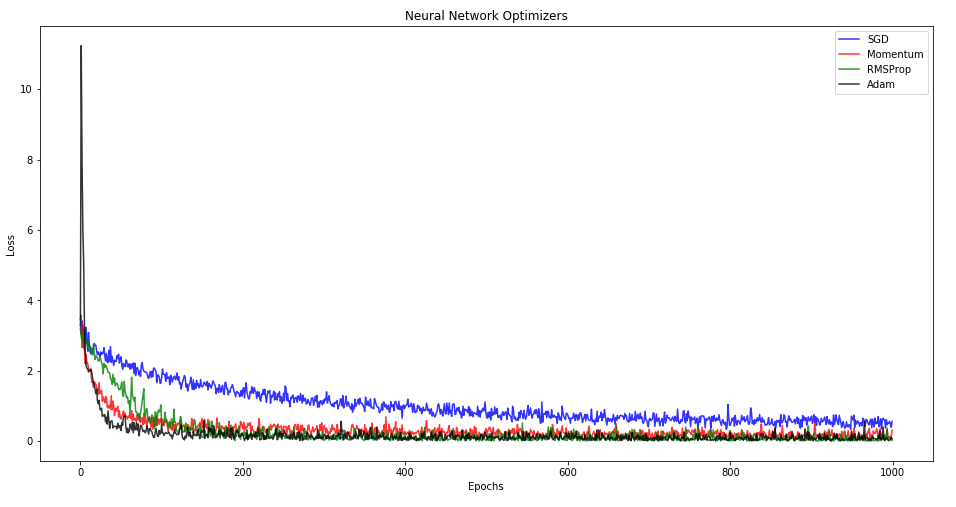
\includegraphics[scale=0.65]{nn_optimizers}

%----------------------------------------------------------------------------------------
%	Introduction - ImageNet Classification
%----------------------------------------------------------------------------------------

\section*{Introduction  - ImageNet Classification}
\hspace{10mm}Current ways to deal with object classification, or object recognition, make basic utilization of machine learning techniques. To enhance their execution, we can gather bigger datasets, take in more powerful models, and utilize better methods for counteracting the process of overfitting. As of not long ago, the datasets of labeled pictures were generally little - on the request of a huge number of pictures (example the NORB dataset, Caltech-101/256 dataset, and CIFAR-10/100 dataset). Basic image recognition errands can be solved great with datasets of this size, particularly on the off chance that they are expanded with name saving changes. For instance, the current best mistake rate on the MNIST digit - classification process (<0.3\%) approaches human execution. \\
\hspace*{10mm}Yet, questions in sensible settings show impressive inconstancy, so to figure out how to remember them it is important to utilize a lot bigger preparing sets. Furthermore, in reality, the inadequacies of little picture datasets have been generally perceived, yet it has as of late turned out to be conceivable to gather marked datasets with a huge number of pictures. The new bigger datasets incorporate LabelMe, which comprises of a huge number of completely sectioned pictures, and ImageNet, which comprises of more than 15 million marked high-goals pictures in more than 22.000 classes. \\
\hspace*{10mm}To find out around a great many items from a huge number of pictures, we require a model with a huge learning limit. Nonetheless, the colossal multifaceted nature of the article acknowledgment errand implies that this issue can't be indicated even by a dataset as expansive as ImageNet, so our model ought to likewise have parts of earlier information to make up for every one of the information we don't have. Convolutional neural networks (CNNs) comprise one such class of models. Their ability can be controlled by fluctuating their profundity and broadness, and they additionally make solid and generally right suspicions about the idea of pictures (in particular, stationarity of measurements and territory of pixel conditions).In this way, contrasted with standard feedforward neural systems with comparatively measured layers, CNNs have many less associations and parameters thus they are less demanding to prepare, while their hypothetically best execution is probably going to be just marginally more regrettable. \\
\hspace*{10mm}Regardless of the alluring characteristics of CNNs, and notwithstanding the overall effectiveness of their neighborhood engineering, they have still been restrictively costly to apply in substantial scale to high-goals pictures. Fortunately, current GPUs, matched with an exceedingly upgraded execution of 2D convolution, are incredible enough to encourage the preparation of curiously vast CNNs, and ongoing datasets, for example, ImageNet contain enough marked guides to prepare such models without serious overfitting. \\
\hspace*{10mm}The explicit commitments of this paper are as per the following: we prepared one of the biggest CNNs to date on the subsets of ImageNet utilized in the ILSVRC-2010 and ILSVRC-2012 rivalries and accomplished by a long shot the best outcomes at any point provided details regarding these datasets. We composed a exceptionally advanced GPU usage of 2D convolution and the various tasks intrinsic in preparing convolutional neural systems, which we make accessible publicly. Our network contains various new and irregular highlights which enhance its execution and lessen its preparation time, which are detailed below. The span of our system made overfitting a critical issue, even with 1.2 million named preparing models, so we utilized a few compelling strategies for averting overfitting, which are portrayed below. Our last system contains five convolutional and three completely associated layers, and this profundity is by all accounts imperative: we found that evacuating any convolutional layer (every one of which contains close to 1\% of the model's parameters) brought about substandard execution. \\
\hspace*{10mm}At last, the system's size is restricted essentially by the measure of memory accessible on current GPUs what's more, by the measure of preparing time that we will endure. Our system takes between five what's more, six days to prepare on two GTX 580 3GB GPUs. The majority of our examinations recommend that our outcomes can be enhanced just by hanging tight for quicker GPUs and greater datasets to end up accessible.

%----------------------------------------------------------------------------------------
%	The Dataset
%----------------------------------------------------------------------------------------

\section*{The Dataset}
\hspace{10mm}ImageNet is a dataset of more than 15 million marked high-goals pictures having a place with around 22.000 classifications. The pictures were gathered from the web and marked by human labelers utilizing Amazon's Mechanical Turk publicly supporting apparatus. Beginning in 2010, as a feature of the Pascal Visual Object Test, a yearly rivalry called the ImageNet Large-Scale Visual Recognition Challenge (ILSVRC) has been held. ILSVRC utilizes a subset of ImageNet with around 1000 pictures in each of 1000 classifications. Altogether, there are generally 1.2 million preparing pictures, 50.000 approval pictures, and 150.000 testing pictures.

%----------------------------------------------------------------------------------------
%	The Architecture
%----------------------------------------------------------------------------------------

\section*{The Architecture}
\hspace{10mm}An illustration of the architecture of our CNN, explicitly showing the delineation of responsibilities between the two GPUs. One GPU runs the layer-parts at the top of the figure while the other runs the layer-parts at the bottom. The GPUs communicate only at certain layers. The network’s input is 150.528-dimensional, and the number of neurons in the network’s remaining layers is given by 253.440–186.624–64.896– 64.896–43.264–4096–4096–1000.
\begin{center}
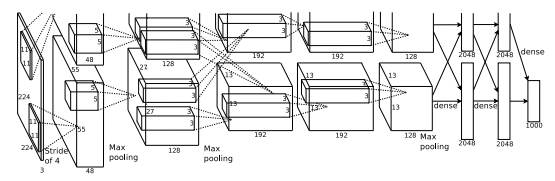
\includegraphics[scale=1]{1}
\end{center}

%----------------------------------------------------------------------------------------
%	Results
%----------------------------------------------------------------------------------------

\section*{Results}
\hspace*{10mm}Our outcomes on ILSVRC-2010 are abridged in Table 1. Our system accomplishes top-1 and best 5 test set mistake rates of 37.5\% and 17.0\%. The best execution accomplished amid the ILSVRC2010 rivalry was 47.1\% and 28.2\% with a methodology that midpoints the forecasts delivered from six meager coding models prepared on various highlights, and from that point forward the best distributed outcomes are 45.7\% and 25.7\% with a methodology that midpoints the expectations of two classifiers prepared on Fisher Vectors (FVs) processed from two kinds of thickly inspected highlights.
\begin{center}
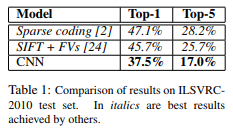
\includegraphics[scale=1]{t1}
\end{center}
\hspace*{10mm}We additionally entered our model in the ILSVRC-2012 rivalry and report our outcomes in Table 2. Since the ILSVRC-2012 test set marks are not freely accessible, we can't report test mistake rates for every one of the models that we attempted. In the rest of this passage, we use approval and test mistake rates reciprocally in light of the fact that as far as we can tell they don't vary by over 0.1\% (see Table 2). The CNN portrayed in this paper accomplishes a best 5 blunder rate of 18.2\%. Averaging the forecasts of five comparative CNNs gives a blunder rate of 16.4\%. Preparing one CNN, with an additional 6th convolutional layer in the course of the last pooling layer, to group the whole ImageNet Fall 2011 discharge (15M pictures, 22K classifications), and afterward "tweaking" it on ILSVRC-2012 gives a mistake rate of 16.6\%. Averaging the forecasts of two CNNs that were pre-prepared on the whole Fall 2011 discharge with the previously mentioned five CNNs gives a blunder rate of 15.3\%. The second-best challenge passage accomplished a mistake rate of 26.2\% with a methodology that midpoints the forecasts of a few classifiers prepared on FVs figured from various kinds of thickly examined highlights.
\begin{center}
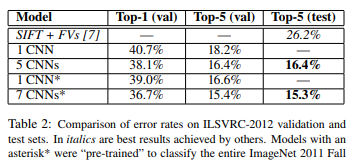
\includegraphics[scale=1]{t2}
\end{center}
\hspace*{10mm}At long last, we likewise report our mistake rates on the Fall 2009 variant of ImageNet with 10,184 classifications furthermore, 8.9 million pictures. On this dataset we pursue the tradition in the writing of utilizing half of the pictures for preparing and half for testing. Since there is no settled test set, our split essentially varies from the parts utilized by past creators, yet this does not influence the outcomes obviously. Our main 1 and best 5 mistake rates on this dataset are 67.4\% and 40.9\%, accomplished by the net depicted above yet with an extra, 6th convolutional layer over the last pooling layer. The best distributed outcomes on this dataset are 78.1\% and 60.9\%.

%----------------------------------------------------------------------------------------
%	Gradient Descent variants
%----------------------------------------------------------------------------------------

\section*{Gradient Descent variants}
\hspace*{10mm}Gradient Descent is an approach to limit a target work $J(\theta)$ parameterized by a model's parameters $\theta \in \mathbb{R}^d$ by refreshing the parameters the other way of the inclination of the target function  with respect to the parameters. The learning rate $\eta$ decides the measure of the steps we take to come to a (neighborhood) least. At the end of the day, we pursue the course of the incline of the surface made by the target work downhill until the point when we come to a valley.\\
\subsection*{Batch gradient descent}
\hspace*{10mm}Vanilla gradient descent, aka batch gradient descent, computes the gradient of the cost function w.r.t.to the parameters $\theta$ for the entire training dataset:
\begin{center}
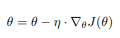
\includegraphics[scale=1]{2}
\end{center}
\hspace*{10mm}As we have to ascertain the gradients for the entire dataset to perform only one refresh, batch gradient descent can be moderate and is unmanageable for datasets that don't fit in memory. Batch gradient descent also does not enable us to refresh our model on the web, i.e. with new models on-the-fly. In code, group angle plummet looks something like:
\begin{center}
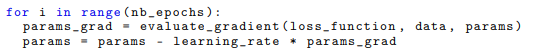
\includegraphics[scale=1]{3}
\end{center}
\subsection*{Stochastic gradient descent}
Stochastic gradient descent (SGD) in contrast performs a parameter update for each training example $x^{(i)}$ and label $y^{(i)}$:
\begin{center}
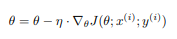
\includegraphics[scale=1]{4}
\end{center}
\begin{center}
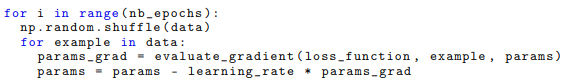
\includegraphics[scale=1]{5}
\end{center}
\subsection*{Mini-batch gradient descent}
\hspace*{10mm}Mini-batch gradient descent finally takes the best of both worlds and performs an update for every mini-batch of n training examples:
\begin{center}
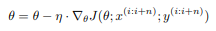
\includegraphics[scale=1]{6}
\end{center}
\hspace*{10mm}Along these lines, it diminishes the difference of the parameter refreshes, which can prompt increasingly stable union and, also, can make utilization of very advanced framework improvements normal to best in class profound learning libraries that make processing the slope w.r.t. a small cluster exceptionally productive. Normal small scale clump sizes extend somewhere in the range of 50 and 256, however can fluctuate for various applications. Smaller than expected clump angle drop is normally the calculation of decision when preparing a neural system and the term Stochastic Gradient Descent normally is utilized likewise when smaller than usual groups are utilized. Note: In adjustments of SGD in the rest of this post, we forget the parameters $x^{(i:i+n)}$; $y^{(i:i+n)}$ for straightforwardness. \\
\hspace*{10mm}In code, rather than repeating over models, we currently emphasize over small scale bunches of size 50:
\begin{center}
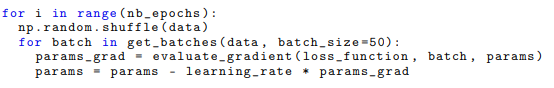
\includegraphics[scale=1]{7}
\end{center}
\hspace*{10mm}There are many Gradient descent optimization algorithms: Momentum, Nesterov accelerated gradient, Adagrad, Adadelta, RMSprop, Adam, AdaMax, Nadam. We can visualize them in the following images
\begin{center}
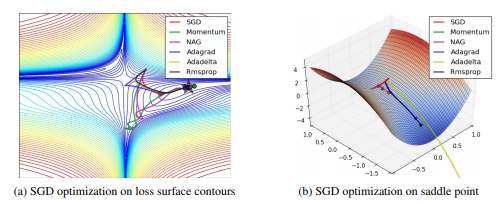
\includegraphics[scale=1]{8}
\end{center}
\subsection*{Which optimizer to use?}
\hspace*{10mm}So, which optimizer should you use? If your input data is sparse, then you likely achieve the best results using one of the adaptive learning-rate methods. An additional benefit is that you will not need to tune the learning rate but will likely achieve the best results with the default value.

%----------------------------------------------------------------------------------------
%	Conclusions
%----------------------------------------------------------------------------------------

\section*{Conclusions}
\hspace*{10mm}The Convolutional Neural Networks are a powerful way to make classification of images. When we create the architecture of a CNN we have to be careful at the size of the dataset. Also, we have to chose a good optimizer for the training step.
%----------------------------------------------------------------------------------------
%	Bibliography
%----------------------------------------------------------------------------------------

\section*{Bibliography} 
\begin{itemize}
	\item \textbf{ImageNet Classification with Deep Convolutional Neural Networks}, Alex Krizhevsky, Ilya Sutskever, Geoffrey E. Hinton.
	\item \textbf{An overview of gradient descent optimization algorithms}, Sebastian Ruder.
	\item \textbf{Large batch training of Convolutional Networks with Layer-wise Adaptive Rate Scaling}, Yang You, Igor Gitman, Boris Ginsburg.
	\item \textbf{Deep Learning}, Ian Goodfellow and Yoshua Bengio and Aaron Courville.
	\item \textbf{Pattern Recognition And Machine Learning}, Christopher M. Bishop.
\end{itemize}

\end{document}
